\chapter{Partial Fractions}

How can you add fractions with different denominators, like $\frac{1}{x} + \frac{2}{x + 3}$? Well, you would need to make the denominators the same, then you could just add the numerators. You achieve this by multiplying the numerator and denominator of each fraction by the denominator of the other fraction:
$$\frac{1}{x} + \frac{2}{x + 3} = \frac{1}{x} \left( \frac{x + 3}{x + 3} \right) + \frac{2}{x + 3} \left( \frac{x}{x} \right)$$

Recall that when the numerator and denominator of a fraction are the same, the fraction is equal to one. So we are not changing the \textit{value} of each fraction, since we are just multiplying by one. Continuing, we can perform the multiplication and see that:
$$\frac{1}{x} + \frac{2}{x + 3} = \frac{x + 3}{x(x + 3)} + \frac{2x}{x(x + 3)}$$
$$= \frac{(x + 3) + 2x}{x(x + 3)} = \frac{3x + 3}{x^2 + 3x} = \frac{3(x + 1)}{x^2 + 3x}$$

The inverse of this process is called \textbf{partial fraction decomposition} (or partial fraction expansion)\index{partial fraction decomposition}. This method has applications in many fields, but we will find it most useful as a tool to evaluate integrals in a later chapter. 


Let $g(x)$ be a rational function such that 
$$g(x) = \frac{P(x)}{Q(x)}$$
Where $P(x)$ and $Q(x)$ are polynomials. If $g(x)$ is proper (that is, the degree of $P$ is less than the degree of $Q$) then we can express $g(x)$ as the sum of simpler rational fractions. If $g(x)$ is improper (that is, the degree of $P$ is greater than or equal to the degree of $Q$), then we must first perform long division to obtain a remainder, $R(x)$, where the degree of $R$ is less than the degree of $Q$:
$$g(x) = \frac{P(x)}{Q(x)} = S(x) + \frac{R(x)}{Q(x)}$$

\subsection{Improper fractions}
What is $\int \frac{x^3 + x}{x-1}\,dx$. Using long division, we see that:
$$\frac{x^3 + x}{x - 1} = x^2 + x + 2 + \frac{2}{x - 1}$$
(see figure \ref{polylongdiv} for an explanation). Then we can also say that:
$$\frac{x^3 + x}{x-1} = x^2 + x + 2 + \frac{2}{x-1}$$

\begin{figure}[htbp]
\centering
    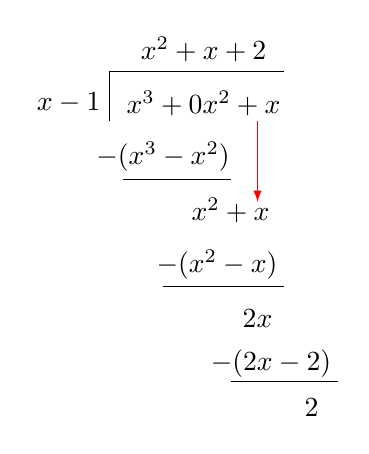
\begin{tikzpicture}
	\begin{axis}[xmin = -1, xmax = 1, axis lines = none, ymin = 0, ymax = 10, clip = false]
            \node[] at (-0.8,8.8) {$x - 1$};
            \draw[black](-0.65, 8.4) -- (-0.65, 9.5);
            \draw[black] (-0.65, 9.5) -- (0, 9.5);
            \node[] at (-0.3, 8.8) {$x^3 + 0x^2 + x$};
            \node[] at (-0.3, 10) {$x^2 + x + 2$};
            \node[] at (-0.45, 7.6) {$-(x^3 - x^2)$};
            \draw[black] (-0.6, 7.1) -- (-0.2, 7.1);
            \node[] at (-0.2, 6.4) {$x^2 + x$};
            \draw[red, -latex](-0.1, 8.4) -- (-0.1, 6.6);
            \node[] at (-0.25, 5.2) {$-(x^2 - x)$};
            \draw[black] (-0.45, 4.7) -- (0, 4.7);
            \node[] at (-0.1, 4) {$2x$};
            \node[] at (-0.05, 3) {$-(2x - 2)$};
            \draw[black] (-0.2, 2.6) -- (0.2, 2.6);
            \node[] at (0.1, 2) {$2$};
        \end{axis}
    \end{tikzpicture}
    \caption{Evaluating $(x^3 + x) \div (x - 1)$ with the long division method}
    \label{polylongdiv}
\end{figure}

When you start with an improper fraction, use long division to reduce it to a 
term plus a proper fraction, then use the methods outlined below to further 
manipulate the proper fraction. 

\begin{Exercise}[label = improper]
Use long division to reduce the following improper rational functions to a term plus a proper rational fraction.
\begin{enumerate}
\item $\frac{x^4 + x^3 + 2x^2 + 2x - 3}{x^2 - 3x + 2}$
\item $\frac{2x^3 + 5}{x^3 - 3x^2 + 2x - 4}$
\item $\frac{3x^4 - 2x^3 - x^2 + 1}{x^3 - 3x}$
\end{enumerate}
\end{Exercise}

\begin{Answer}[ref = improper]

\end{Answer}

\subsection{Proper fractions}
When the order of the numerator is less than or equal to the denominator, 
there are three further possibilities. 

\subsubsection{No repeated linear factors}
In the first case, the denominator, $Q(x)$ is composed of distinct linear 
factors. In this case, we can say that $Q(x) = (a_1x + b_1)(a_2x + b_2) \cdots 
(a_nx + b_n)$, where no factor is repeated (including constant multiples). 
Then, there exists $A, B, C, \cdots$ such that:
$$\frac{P(x)}{Q(x)} = \frac{A}{a_1x+b_1} + \frac{B}{a_2x + b_2} + \cdots$$

Let's see an example of this by decomposing $\frac{4x^2 - 7x - 12}{x (x + 2) (x 
- 3)}$. We start by defining $A$, $B$, and $C$, such that:
$$\frac{4x^2 - 7x - 12}{x (x + 2) (x - 3)} = \frac{A}{x} + \frac{B}{x + 2} + 
\frac{C}{x - 3}$$
Multiplying both sides by $x (x + 2) (x - 3)$ we get:
$$4x^2 - 7x - 12 = A(x + 2)(x - 3) + B(x)(x - 3) + C(x)(x + 2)$$
We have 3 unknowns and only one equation! Don't worry: remember this equation 
is true for all $x$, so we can choose a convenient value of $x$ to isolate 
each unknown in turn. Starting, let $x = 0$. Then:
$$4(0)^2 - 7(0) - 12 = A(0 + 2)(0 - 3) + B(0)(x - 3) + C(0)(x + 2)$$
$$-12 = A(2)(-3) + 0 + 0$$
Notice that the $B$ and $C$ disappear, and we can solve for $A$:
$$A = \frac{-12}{-6} = 2$$
We can solve for $B$ by setting $x = -2$ and for $C$ by setting $x = 3$ 
(notice, we've used all three zeroes of the denominator polynomial):
$$4(-2)^2 - 7(-2) - 12 = A(-2 + 2)(-2 - 3) + B(-2)(-2 - 3) + C(-2)(-2 + 2)$$
$$4(4) + 14 - 12 = 0 + B(-2)(-5) + 0$$
$$16 + 2 = 10B$$
$$B = \frac{9}{5}$$
and
$$4(3)^2 - 7(3) - 12 = A(3 + 2)(3 - 3) + B(3)(3 - 3) + C(3)(3 + 2)$$
$$4(9) - 21 - 12 = 0 + 0 + C(3)(5)$$
$$36 - 33 = 15C$$
$$C = \frac{1}{5}$$
And we can decompose our original fraction:
$$\frac{4x^2 - 7x - 12}{x (x + 2) (x - 3)} = \frac{2}{x} + \frac{9}{5(x + 2)} 
+ \frac{1}{5(x - 3)}$$
You can check your answer by cross-multiplying and adding. You should get the 
same rational function back. 

\subsubsection{Repeated linear factors}
The second case is if $Q(x)$ has repeated factors (such as $x^2 + 8x + 16 = (x 
+ 4)^2$). Suppose the first linear factor, $(a_1x + b_1)$ is repeated $r$ 
times (that is, $Q(x)$ contains the factor $(a_1x + b_1)^r$). Then instead of 
$\frac{A}{a_1x + b_1}$ we should write:
$$\frac{A_1}{a_1x + b_1} + \frac{A_2}{(a_1x + b_1)^2} + \cdots + \frac{A_r}{(
a_1x + b_1)^r}$$
Let's look at a concrete example to see how this works:

\textbf{Example}: Decompose $\frac{x^2 + x + 1}{(x + 1)^2 (x + 2)}$

\textbf{Solution}: We start by defining:
$$\frac{x^2 + x + 1}{(x + 1)^2 (x + 2)} = \frac{A}{x + 1} + \frac{B}{(x + 1)^
2} + \frac{C}{x + 2}$$
Multiplying both sides by $(x + 1)^2 (x + 2)$:
$$x^2 + x + 1 = A(x + 1)(x + 2) + B(x + 2) + C(x + 1)^2$$
Since there are only 2 roots to $(x + 1)^2 (x + 2)$, we will use another 
method called ''equating the coefficients" to find $A$, $B$, and $C$. We start 
by expanding the right side of the equation:
$$x^2 + x + 1 = A(x^2 + 3x + 2) + B(x + 2) + C(x^2 + 2x + 1)$$
Distributing and combining, we find that:
$$x^2 + x + 1 = Ax^2 + 3Ax + 2A + Bx + 2B + Cx^2 + 2Cx + C$$
$$x^2 + x + 1 = (A + C)x^2 + (3A + B + 2C)x + (2A + 2B + C)$$
For this equation to be true, we know that:
$$A + C = 1$$
$$3A + B + 2C = 1$$
$$2A + 2B + C = 1$$
(That is, the coefficient for $x^2$ on the left, 1, must be equal to the 
coefficient for $x^2$ on the right, (A + C), and so on.) We now have a system 
of 3 equations and 3 unknowns. When you solve for each, you should find that:
$$A = -2$$
$$B = 1$$
$$C = 3$$
And therefore, 
$$\frac{x^2 + x + 1}{(x + 1)^2 (x + 2)} = \frac{-2}{x + 1} + \frac{1}{(x + 1)^
2} + \frac{3}{x + 2}$$

\subsubsection{Irreducible quadratic factors}
Sometimes we cannot express a polynomial as the product of two linear 
statements (that is, terms in the form $ax + b$). Take $x^2 + 1$, which 
cannot be expressed as the product of real, linear terms. What do you do 
if something like $x^2 + 1$ is in the denominator? Then when we write an 
expression for $\frac{P(x)}{Q(x)}$ we include a term in the form:
$$\frac{Ax + B}{ax^2 + bx + c}$$
For example, we can write
$$\frac{x}{(x - 2)(x^2 + 1)(x^2 + 4)} = \frac{A}{x - 2} + \frac{Bx + C}{x^2 + 1} 
+ \frac{Dx + E}{x^2 + 4}$$

\textbf{Example}: Decompose $\frac{2x^2 - x + 4}{x^3 + 4x}$

\textbf{Solution}: We begin by factoring the denominator:
$$x^3 + 4x = x(x^2 + 4)$$
Which cannot be factored further. Therefore, we define:
$$\frac{2x^2 - x + 4}{x(x^2 + 4)} = \frac{A}{x} + \frac{Bx + C}{x^2 + 4}$$
$$2x^2 - x + 4 = A(x^2 + 4) + (Bx + C)x$$
$$2x^2 - x + 4 = Ax^2 + 4A + Bx^2 + Cx$$
Which implies that:
$$2 = A + B$$
$$C = -1$$
$$4A = 4$$
Therefore, $A = 1$, $B = 1$, and $C = -1$ and we can say that:
$$\frac{2x^2 - x + 4}{x^3 + 4x} = \frac{1}{x} + \frac{x - 1}{x^2 + 4}$$

\subsubsection{Repeated irreducible quadratic factors}
Lastly, the denominator might contain repeated irreducible quadratic factors. 
Similar to repeated linear factors, when setting up your partial fractions, 
instead of only writing 
$$\frac{A}{ax^2 + bx + c}$$
For a quadratic factor that is repeated $r$ times, your equation should include:
$$\frac{A_1}{ax^2 + bx + c} + \frac{A_2}{(ax^2 + bx + c)^2} + \cdots + 
\frac{A_r}{(ax^2 + bx + c)^r}$$